\documentclass[12pt,a4paper] {article} 
\usepackage{hyperref}
\usepackage{graphicx}
\usepackage{url}
\usepackage{amssymb}
\usepackage{breakcites}
\usepackage{dirtytalk}

\usepackage{filecontents}
\begin{filecontents}{Proposal.bib}
	@misc{pubmed,
		author = {National Center for Biotechnology Information},
		title = {PubMed},
		howpublished = {\url{https://www.ncbi.nlm.nih.gov/pubmed}}
	}
	
	@misc{annoy,
		author = {Github},
		title = {Annoy},
		howpublished = {\url{https://github.com/spotify/annoy}}
	}
	
	
	
	@misc{selenium,
		author = {Selenium Web driver},
		title = {Selenium},
		howpublished = {\url{http://www.seleniumhq.org/docs/03_webdriver.jsp }}
	}
	@inproceedings{le2014distributed,
		title={Distributed representations of sentences and documents},
		author={Le, Quoc and Mikolov, Tomas},
		booktitle={Proceedings of the 31st International Conference on Machine Learning (ICML-14)},
		pages={1188--1196},
		year={2014}
	}
	
	
	
	
	@Inbook{Bengio2006,
		author="Bengio, Yoshua
		and Schwenk, Holger
		and Sen{\'e}cal, Jean-S{\'e}bastien
		and Morin, Fr{\'e}deric
		and Gauvain, Jean-Luc",
		editor="Holmes, Dawn E.
		and Jain, Lakhmi C.",
		title="Neural Probabilistic Language Models",
		bookTitle="Innovations in Machine Learning: Theory and Applications",
		year="2006",
		publisher="Springer Berlin Heidelberg",
		address="Berlin, Heidelberg",
		pages="137--186",
		abstract="A central goal of statistical language modeling is to learn the joint probability function of sequences of words in a language. This is intrinsically difficult because of the curse of dimensionality: a word sequence on which the model will be tested is likely to be different from all the word sequences seen during training. Traditional but very successful approaches based on n-grams obtain generalization by concatenating very short overlapping sequences seen in the training set. We propose to fight the curse of dimensionality by learning a distributed representation for words which allows each training sentence to inform the model about an exponential number of semantically neighboring sentences. Generalization is obtained because a sequence of words that have never been seen before gets high probability if it is made of words that are similar (in the sense of having a nearby representation) to words forming an already seen sentence. Training such large models (with millions of parameters) within a reasonable time is itself a significant challenge. We report on several methods to speed-up both training and probability computation, as well as comparative experiments to evaluate the improvements brought by these techniques. We finally describe the incorporation of this new language model into a state-of-the-art speech recognizer of conversational speech.",
		isbn="978-3-540-33486-6",
		doi="10.1007/3-540-33486-6_6",
		url="https://doi.org/10.1007/3-540-33486-6_6"
	}
	
	@article{mikolov2013efficient,
		title={Efficient estimation of word representations in vector space},
		author={Mikolov, Tomas and Chen, Kai and Corrado, Greg and Dean, Jeffrey},
		journal={arXiv preprint arXiv:1301.3781},
		year={2013}
	}
	
	
	@inproceedings{pennington2014glove,
		title={Glove: Global vectors for word representation},
		author={Pennington, Jeffrey and Socher, Richard and Manning, Christopher},
		booktitle={Proceedings of the 2014 conference on empirical methods in natural language processing (EMNLP)},
		pages={1532--1543},
		year={2014}
	}
	
	@article{robertson2009probabilistic,
		title={The probabilistic relevance framework: BM25 and beyond},
		author={Robertson, Stephen and Zaragoza, Hugo and others},
		journal={Foundations and Trends{\textregistered} in Information Retrieval},
		volume={3},
		number={4},
		pages={333--389},
		year={2009},
		publisher={Now Publishers, Inc.}
	}
	
	
	@article{chen2017efficient,
		title={Efficient vector representation for documents through corruption},
		author={Chen, Minmin},
		journal={arXiv preprint arXiv:1707.02377},
		year={2017}
	}
	
	@article{collobert2011natural,
		title={Natural language processing (almost) from scratch},
		author={Collobert, Ronan and Weston, Jason and Bottou, L{\'e}on and Karlen, Michael and Kavukcuoglu, Koray and Kuksa, Pavel},
		journal={Journal of Machine Learning Research},
		volume={12},
		number={Aug},
		pages={2493--2537},
		year={2011}
	}
	
	
	@article{mitchell2010composition,
		title={Composition in distributional models of semantics},
		author={Mitchell, Jeff and Lapata, Mirella},
		journal={Cognitive science},
		volume={34},
		number={8},
		pages={1388--1429},
		year={2010},
		publisher={Wiley Online Library}
	}
	
	
	@inproceedings{zanzotto2010estimating,
		title={Estimating linear models for compositional distributional semantics},
		author={Zanzotto, Fabio Massimo and Korkontzelos, Ioannis and Fallucchi, Francesca and Manandhar, Suresh},
		booktitle={Proceedings of the 23rd International Conference on Computational Linguistics},
		pages={1263--1271},
		year={2010},
		organization={Association for Computational Linguistics}
	}
	
	@inproceedings{yessenalina2011compositional,
		title={Compositional matrix-space models for sentiment analysis},
		author={Yessenalina, Ainur and Cardie, Claire},
		booktitle={Proceedings of the Conference on Empirical Methods in Natural Language Processing},
		pages={172--182},
		year={2011},
		organization={Association for Computational Linguistics}
	}
	
	@article{grefenstette2013multi,
		title={Multi-step regression learning for compositional distributional semantics},
		author={Grefenstette, Edward and Dinu, Georgiana and Zhang, Yao-Zhong and Sadrzadeh, Mehrnoosh and Baroni, Marco},
		journal={arXiv preprint arXiv:1301.6939},
		year={2013}
	}
	
	@inproceedings{mikolov2013distributed,
		title={Distributed representations of words and phrases and their compositionality},
		author={Mikolov, Tomas and Sutskever, Ilya and Chen, Kai and Corrado, Greg S and Dean, Jeff},
		booktitle={Advances in neural information processing systems},
		pages={3111--3119},
		year={2013}
	}
	
	@inproceedings{socher2011dynamic,
		title={Dynamic pooling and unfolding recursive autoencoders for paraphrase detection},
		author={Socher, Richard and Huang, Eric H and Pennin, Jeffrey and Manning, Christopher D and Ng, Andrew Y},
		booktitle={Advances in Neural Information Processing Systems},
		pages={801--809},
		year={2011}
	}
	
	@article{mitra2016dual,
		title={A dual embedding space model for document ranking},
		author={Mitra, Bhaskar and Nalisnick, Eric and Craswell, Nick and Caruana, Rich},
		journal={arXiv preprint arXiv:1602.01137},
		year={2016}
	}
	
	
	@article{blei2003latent,
		title={Latent dirichlet allocation},
		author={Blei, David M and Ng, Andrew Y and Jordan, Michael I},
		journal={Journal of machine Learning research},
		volume={3},
		number={Jan},
		pages={993--1022},
		year={2003}
	}
	
	
	@inproceedings{ghosh2016characterizing,
		title={Characterizing diseases from unstructured text: A vocabulary driven word2vec approach},
		author={Ghosh, Saurav and Chakraborty, Prithwish and Cohn, Emily and Brownstein, John S and Ramakrishnan, Naren},
		booktitle={Proceedings of the 25th ACM International on Conference on Information and Knowledge Management},
		pages={1129--1138},
		year={2016},
		organization={ACM}
	}
	
	@article{joulin2016bag,
		title={Bag of tricks for efficient text classification},
		author={Joulin, Armand and Grave, Edouard and Bojanowski, Piotr and Mikolov, Tomas},
		journal={arXiv preprint arXiv:1607.01759},
		year={2016}
	}
	
	@article{sidorov2014soft,
		title={Soft similarity and soft cosine measure: Similarity of features in vector space model},
		author={Sidorov, Grigori and Gelbukh, Alexander and G{\'o}mez-Adorno, Helena and Pinto, David},
		journal={Computaci{\'o}n y Sistemas},
		volume={18},
		number={3},
		pages={491--504},
		year={2014},
		publisher={Centro de Investigaci{\'o}n en Computaci{\'o}n, IPN}
	}
	
	@inproceedings{kusner2015word,
		title={From word embeddings to document distances},
		author={Kusner, Matt and Sun, Yu and Kolkin, Nicholas and Weinberger, Kilian},
		booktitle={International Conference on Machine Learning},
		pages={957--966},
		year={2015}
	}
	
	
	@inproceedings{rehurek_lrec,
		title = {{Software Framework for Topic Modelling with Large Corpora}},
		author = {Radim {\v R}eh{\r u}{\v r}ek and Petr Sojka},
		booktitle = {{Proceedings of the LREC 2010 Workshop on New
				Challenges for NLP Frameworks}},
		pages = {45--50},
		year = 2010,
		month = May,
		day = 22,
		publisher = {ELRA},
		address = {Valletta, Malta},
		note={\url{http://is.muni.cz/publication/884893/en}},
		language={English}
	}
	
\end{filecontents}

\begin{document}
	
	\title{Semantic Similarity in Medical Domain \\ \hphantom \newline
		\large     Expos\'{e} of Master Thesis
		\\Bonn University \& Fraunhofer IAIS}
	\author{Abbas Goher}
	\date{February, 2018, St. Augustin}
	\maketitle
	
	The goal of this thesis is to use a neural network model to map patient records to semantically similar and potentially helpful research work. For training the model large volume of raw texts from PubMed \cite{pubmed}  will be used.
	
	
	The traditional approach for finding relevant documents for a given query is to count repetitions of query terms in the documents. Different weight schemes for these counts lead to a variety of TF-IDF ranking features. However, the basic forms of such a ranking system only consider query terms, under the assumption that non-query terms are less useful for document ranking. This makes such ranking systems incapable of capturing the deep semantic meaning of the text all by itself. 
	
	Neural network models have recently shown impressive results in capturing the underlying semantics of the documents\cite{Bengio2006}.
	The main stumbling block in creating such a semantic model is the lack of labeled data required for training such a method. Another challenge is the lack of freely available data, PubMed mostly provides abstracts of research articles for free. 
	
	The main idea of this thesis is to explore ways in which deep learning can be used for solving the problem of finding semantically similar/helpful research articles given a patient record. The chosen direction of the research is to apply Doc2Vec model proposed in \cite{le2014distributed} and explore different ways in which the Doc2Vec model can be extended/improved.
	
	\section*{Background \& Literature Review}
	
	\subsection*{Embedding Models}
	Usage of deep learning in the context of NLP tasks requires representing the text as the input for neural networks. As of late, the most used and powerful representations are one of the following embeddings: Word2Vec \cite{mikolov2013efficient} and GloVe \cite{pennington2014glove}, which are word level embeddings. An extension to Word2Vec known as Doc2Vec was proposed in \cite{le2014distributed}.  
	
	We look closer at the Word2Vec and Doc2Vec models, as they are the most relevant to this work. Word2Vec model uses distributed vector representation of words, a well-known framework for learning word vectors as shown in the Figure 1. The task is to learn to predict a word given other words in the context.
	More formally, given a sequence of training words
	$w_{1}, w_{2}, w_{3}, ..., w_{T} $, the objective of the word vector model is to maximize the average log probability
	\\
	\begin{equation}
	\frac{1}{T} \sum_{t=K}^{T-K} \log p(w_{t} \mid w_{t-1},....,w_{t+1}) 
	\end{equation}
	
	\begin{figure}[h]
		\centering
		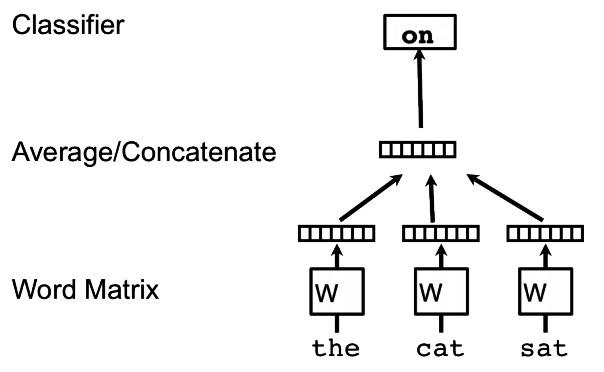
\includegraphics[width=8cm, height=5cm]{w2v.png}
		\caption[]{A framework for learning word vectors. Context of
			three words (“the,” “cat,” and “sat”) is used to predict the fourth
			word (“on”). The input words are mapped to columns of the matrix
			W to predict the output word.}
		\label{fig:Word2Vec model}
	\end{figure}
	Some commendable efforts have been made to go beyond word level representations  \cite{mitchell2010composition}  \cite{zanzotto2010estimating} 
	\cite{yessenalina2011compositional}  \cite{grefenstette2013multi}  \cite{mikolov2013distributed}. A simple approach is to use the weighted average of all the words in the document. But weighted averaging of word vectors loses the word order. A more sophisticated approach is combining the word vectors
	in an order given by a parse tree of a sentence, using
	matrix-vector operations \cite{socher2011dynamic}. A drawback of such an approach is that it only works on sentences as it relies on parse trees.
	
	Doc2Vec is capable of constructing representations
	of input sequences of variable length. Unlike some of the
	previous approaches, it is general and applicable to texts of
	any length: sentences, paragraphs, and documents. In Doc2Vec framework (see Figure 2), every
	document is mapped to a unique vector, and every word is also mapped to a
	unique vector. The document vector and word vectors are averaged or concatenated
	to predict the next word in a context. The only difference to a Word2Vec model is the additional document token.It
	acts as a memory that remembers what is missing from the
	current context – or the topic of the document. The document vectors and word vectors are trained using stochastic gradient descent and the gradient is obtained via back-propagation.
	
	
	\begin{figure}[h]
		\centering
		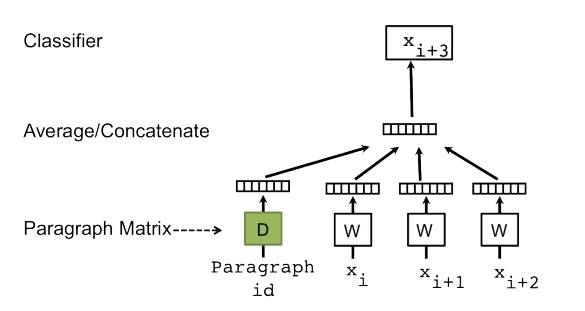
\includegraphics[width=8cm, height=5cm]{para}
		\caption[]{A framework for learning paragraph vector. This framework
			is similar to the framework presented in Figure 1; the only
			change is the additional paragraph token that is mapped to a vector
			via matrix D. In this model, the concatenation or average of
			this vector with a context of three words is used to predict the
			fourth word. The paragraph vector represents the missing information
			from the current context and can act as a memory of the
			topic of the paragraph.}
		\label{fig:doc2vec model}
	\end{figure}
	
	\subsection*{Embedding Model Extension}
	
	Classical emitting methods such as Doc2Vec and Word2Vec are generally unsupervised requiring no domain information and as such has broad
	applicability. However, for highly specified domains with a moderately sized corpus, classical methods fail to find meaningful semantic relationships. 
	\cite{ghosh2016characterizing} introduce a vocabulary driven Word2Vec method known as Dis2Vec which is used to generate disease-specific word embeddings from unstructured health-related news corpus. The input corpus $D$ consists of a collection of word context pairs. Based on the vocabulary $ V$, we can categorize the word context pairs into three types as shown
	below:
	\\
	\begin{itemize}
		\item $ D(d) = {(w, c): w \in V ∧c \in V }$, i.e. both the word w and the context c are in V
		\item $D(\rightharpoondown d) = {(w, c): w \notin V ∧c \notin V }$, i.e. neither the word w nor the context c are in V
		\item $D(\rightharpoondown d) = {(w, c): w \in V \oplus c \in V }$, i.e. either the word w is in V or the context c is in V but both cannot be in V
	\end{itemize}
	
		
	
	\section*{Planned work} 
	The work is planned to consist of the following stages:
	\begin{itemize}
		\item Use the gensim \cite{rehurek_lrec} implementation of the Doc2Vec model as described in (\cite{le2014distributed}), and train it on
		the following
		\begin{itemize}
			\item Full Wikipedia articles 
			\item Wikipedia info-boxes
			\item A smaller subset of PubMed only containing only  colorectal cancer abstracts
			\item Full PubMed abstracts
			\item PMC another Subset of PubMed which contains full articles
		\end{itemize}
		
		
		\item Manual preprocessing
		\begin{itemize}
			\item PubMed uses special language/notation to describe different age-groups. i.e elderly, middle-aged, $>$60 years old and 50-60 years old. Similar language/notation will be used while generating patient descriptions from a given database.
			
			\item Extending the query document by adding rephrases of the key parts. For example, The query document \say {75 years old patient has rectal cancer } is extended to \say{ Elderly patient, $>$70 years old, The patient has rectal cancer, cancer in rectum }. The query document is generated in a structured way to allow an easy extension. The basic structure of the query document is \say{Age, Gender, Type of cancer, Type of metastasis}.
			 
			\item Instead of generating the full patient record, only the following information is recorded
			\begin{itemize}
				\item The type of cancer
				\item Patients age
				\item Patients gender
				\item Primary tumor location
				\item Type of surgery to be performed
				
			\end{itemize} 
			
		\end{itemize}
		

		\item Use different variants of Doc2Vec like DBOW, DM and DMC to see which performs the best.
		
		
		\item Extend the Dis2Vec \cite{ghosh2016characterizing} model to work on document level.
		
		\item Use different distance metrics such as \cite{sidorov2014soft} \cite{kusner2015word} and \cite{annoy} to find out which distance metric produces the best results.
		
		\item Compare the final results against the vanilla Doc2Vec model.
		
		
	\end{itemize}
	
	
	
	\section*{Technical Description} 
	\subsection*{Implementation}
	The Following tools are to be used in the project
	
	\begin{itemize}
		\item Gensim library \cite{rehurek_lrec} implementation will be used for the vanilla Doc2vec model and its variants. 
		
		\item Pythons nltk library will be used for tokenization and stop-word removal
		
		\item Python library regex will be used for parsing the full PubMed abstracts 
		
		\item To reduce the training time some elements will be implemented in Cython. Cython file will then be used to generate a .c file for faster computation
		
		\item GCC 4.9 compiler will be used to compile the .c file generated by Cython 
		
		
	\end{itemize}
	
	
	\subsection*{Datasets}
	For the basic research on the quality of the network, the following datasets can 
	be used:
	\begin{itemize}
		\item Wikipedia articles corpus
		\item Wikipedia info-box corpus
	\end{itemize}
	
	For medical domain, the following can be used:
	\begin{itemize}
		\item Pubmed abstracts subset corpus on colorectal cancer
		\item Full set of Pubmed abstracts
		\item PMC, another subset of PubMed which contains full articles
	\end{itemize}
	
	
	\subsection*{Validation}
	
	\subsubsection*{Wikipedia and Info-box corpus}
	Following steps describe the technique to be used as a proof of method on Full Wikipedia corpus and Wikipedia info-box corpus. 
	
	\begin{itemize}
		
		
		
		\item Take a random target article and use the part of its information to infer a vector. Infer-vector is a method to obtain an embedding for the out-of-sample documents. Inference starts with a low-magnitude random vector, that is then incrementally adjusted to be more predictive.
		
		\item Use this inferred vector to find 10 similar documents.
		\item The prediction task is to predict the article the given information belongs to.
		
	\end{itemize}
	
	
	Initial experiments revealed an interesting correlation between the size of the document and the number of iterations (a.k.a steps)  used to infer a vector.
	
	\subsubsection*{PubMed corpus}
	
	For the medical domain, we first infer a vector for a patient description and then find PubMed abstracts which are semantically closer to the given patient record.
	For result evaluation, we have 400 labeled abstracts. For each of these 400 abstracts, we have 10 other abstracts which have been labeled to be semantically close. 
	
	For a given query document the task is to predict semantically similar documents.
	
	
	
	\subsection*{Evaluation Metric}
	Precision and recall are single-value metrics based on the whole list of documents returned by the system. For systems that return a ranked sequence of documents, it is desirable to also consider the order in which the returned documents are presented. Average Precision(AP) is thus define as:
	
	\begin{equation}
	AP =\frac {\sum_{k=1}^{n}(P(k)\times rel (k))}{\mbox {number of relevant documents}}
	\end{equation}
	
	where k is the rank in the sequence of retrieved documents,  n is the number of retrieved documents,  P(k) is the precision at cut-off k in the list and rel(k) is an indicator function equaling 1 if the item at rank k is a relevant document, zero otherwise.
	
	For multiple queries, an extension of average precision known as mean average precision is used. Mean average precision for a set of queries is the mean of the average precision scores for each query. In this thesis mean average precision(MAP) will be used as an evaluation metric.
	
	\bibliographystyle{abbrv}
	\bibliography{Proposal} 
	
\end{document}
